% =====================================================================
%  Cerebro Cuantico Optogenetico -- Teoria detallada del modelo
%  Compilar con:  pdflatex teoria_cerebro_cuantico.tex  (dos veces)
%  Figuras en:    figuras/  (generadas con el codigo de qollab/cerebro_q)
% =====================================================================
\documentclass[11pt,a4paper]{article}

\usepackage[utf8]{inputenc}
\IfFileExists{lmodern.sty}{\usepackage{lmodern}\usepackage[T1]{fontenc}}{}
\IfFileExists{spanish.ldf}%
  {\usepackage[spanish,es-noshorthands,es-tabla,es-nodecimaldot]{babel}}%
  {\usepackage[english]{babel}% respaldo si falta el castellano: mismos nombres
   \addto\captionsenglish{\renewcommand{\figurename}{Figura}\renewcommand{\tablename}{Tabla}%
     \renewcommand{\contentsname}{Índice}\renewcommand{\abstractname}{Resumen}%
     \renewcommand{\refname}{Referencias}\renewcommand{\appendixname}{Apéndice}}}
\usepackage[margin=2.5cm]{geometry}
\usepackage{amsmath,amssymb,amsthm,mathtools}
\usepackage{bm}
\usepackage{graphicx}
\usepackage{booktabs}
\usepackage{array}
\newcolumntype{L}[1]{>{\raggedright\arraybackslash}p{#1}}
\usepackage{xcolor}
\usepackage{tikz}
\usetikzlibrary{arrows.meta,positioning,shapes.geometric,fit,calc}
\usepackage{quantikz}
\usepackage{listings}
\usepackage[most]{tcolorbox}
\usepackage[expansion=false]{microtype}
\usepackage[hidelinks]{hyperref}
\usepackage{cleveref}

% ---------------------------------------------------------------- colores
\definecolor{azul}{HTML}{2A78D6}
\definecolor{naranjo}{HTML}{EB6834}
\definecolor{verde}{HTML}{1BAF7A}
\definecolor{violeta}{HTML}{6250D6}
\definecolor{tinta}{HTML}{52514E}

% ---------------------------------------------------------------- notación
% quantikz ya define \ket y \bra; se redefinen con la misma notación
\renewcommand{\ket}[1]{\lvert #1\rangle}
\renewcommand{\bra}[1]{\langle #1\rvert}
\newcommand{\bk}[2]{\langle #1\vert #2\rangle}
\renewcommand{\proj}[1]{\lvert #1\rangle\!\langle #1\rvert}
\newcommand{\vac}{\ket{\mathbf{0}}}
\newcommand{\e}{\mathrm{e}}
\newcommand{\ii}{\mathrm{i}}
\newcommand{\tr}{\operatorname{Tr}}
\newcommand{\hop}{\mathrm{hop}}
\newcommand{\TVD}{\mathrm{TVD}}
\newcommand{\Nop}{\hat N}
\newcommand{\RX}{R_X}
\newcommand{\RXX}{R_{XX}}
\newcommand{\RYY}{R_{YY}}
\newcommand{\code}[1]{\texttt{#1}}

% ---------------------------------------------------------------- teoremas
\theoremstyle{plain}
\newtheorem{proposicion}{Proposición}[section]
\newtheorem{lema}[proposicion]{Lema}
\theoremstyle{definition}
\newtheorem{definicion}[proposicion]{Definición}
\theoremstyle{remark}
\newtheorem*{observacion}{Observación}
\renewcommand{\proofname}{Demostración}
\AtBeginDocument{%
  \renewcommand{\crefpairconjunction}{ y }%
  \renewcommand{\crefmiddleconjunction}{, }%
  \renewcommand{\creflastconjunction}{ y }%
  \renewcommand{\crefpairgroupconjunction}{ y }%
  \renewcommand{\crefmiddlegroupconjunction}{, }%
  \renewcommand{\creflastgroupconjunction}{ y }%
  \renewcommand{\crefrangeconjunction}{ a }}
\crefname{proposicion}{proposición}{proposiciones}
\crefname{lema}{lema}{lemas}
\crefname{definicion}{definición}{definiciones}
\crefname{figure}{figura}{figuras}
\crefname{table}{tabla}{tablas}
\crefname{section}{sección}{secciones}
\crefname{subsection}{sección}{secciones}
\crefname{equation}{ec.}{ecs.}
\crefname{appendix}{apéndice}{apéndices}

% ---------------------------------------------------------------- cajas
\newtcolorbox{idea}[1][]{colback=azul!5,colframe=azul!70,boxrule=0.6pt,arc=2pt,
  left=6pt,right=6pt,top=4pt,bottom=4pt,fonttitle=\bfseries,title={#1}}
\newtcolorbox{honestidad}{colback=naranjo!6,colframe=naranjo!80,boxrule=0.6pt,arc=2pt,
  left=6pt,right=6pt,top=4pt,bottom=4pt,fonttitle=\bfseries,title={Límite del modelo}}

\lstset{basicstyle=\ttfamily\small,columns=fullflexible,keepspaces=true,
  frame=single,rulecolor=\color{tinta!40},backgroundcolor=\color{tinta!4},
  keywordstyle=\color{azul}\bfseries,commentstyle=\color{tinta}\itshape,
  language=Python,showstringspaces=false,xleftmargin=4pt,xrightmargin=4pt}

\title{\textbf{Cerebro Cuántico Optogenético}\\[4pt]
\large Teoría detallada: del conectoma de \emph{C.~elegans} a un circuito de Qiskit}
\author{Documento de estudio del equipo}
\date{Octubre de 2026}

\begin{document}
\maketitle

\begin{abstract}
\noindent
Este documento explica, con todas las demostraciones, la física detrás del proyecto. Cada una de las 302 neuronas de \emph{C.~elegans} se representa con un qubit. Las sinapsis reales del gusano definen un hamiltoniano de saltos tipo XY, y un pulso de luz (el ``láser optogenético'') es una rotación $\RX(\theta)$ sobre la neurona iluminada. Se demuestra que, con un láser, la dinámica es \emph{exactamente} un \emph{quantum walk} de tiempo continuo sobre el conectoma. De ahí sale el resultado central, $P_k(t)=\sin^2(\theta/2)\,\bigl|[\e^{-\ii\gamma J t}]_{kj}\bigr|^2$. Después se construye el circuito que lo simula: fórmulas de Trotter--Suzuki y su error, cascada de Givens, compilación a las compuertas nativas de IonQ, modelo de ruido, presupuesto de errores y mitigación por post-selección de simetría. Todas las cifras y figuras se calcularon con el mismo código del proyecto (\code{qollab/cerebro\_q}).
\end{abstract}

\begin{honestidad}
\textbf{Nota de versión.} Este documento largo se escribió cuando el proyecto usaba pesos logarítmicos, $W_{ij}=\log(1+n_{ij})$. El equipo pasó después a pesos binarios (todas las sinapsis pesan igual). Las derivaciones valen igual para cualquier $J$ simétrica; las cifras concretas de este texto ($\lambda_{\max}$, TVD, fidelidades) corresponden a los pesos logarítmicos. Los valores actuales están en \code{teoria\_cerebro\_cuantico.tex}, y si se recompila este archivo las figuras saldrán ya con pesos binarios.
\end{honestidad}

\tableofcontents
\newpage

% =====================================================================
\section{Motivación y alcance}
\label{sec:motivacion}
% =====================================================================

\subsection{La idea en una página}

La \emph{optogenética} controla neuronas con luz. Se expresa en ellas una proteína sensible a la luz, como la channelrhodopsina-2 (ChR2), que abre un canal iónico al recibir luz azul ($\sim470$\,nm)~\cite{boyden2005}. Un pulso de luz puede así hacer ``disparar'' una neurona concreta, y se observa cómo la actividad se propaga por la red. En el nematodo \emph{Caenorhabditis elegans}, iluminar los receptores de toque que expresan ChR2 provoca la respuesta de escape del animal~\cite{nagel2005}. Este gusano es el único animal adulto con el conectoma completo descrito: 302 neuronas y todas sus sinapsis~\cite{white1986,cook2019}.

El proyecto traduce ese experimento al lenguaje de la computación cuántica:

\begin{center}
\renewcommand{\arraystretch}{1.25}
\begin{tabular}{@{}L{0.44\textwidth}L{0.48\textwidth}@{}}
\toprule
\textbf{Optogenética real} & \textbf{Este modelo} \\
\midrule
Neurona en reposo / activa & Qubit en $\ket{0}$ / $\ket{1}$ \\
Pulso de luz que abre la ChR2 & Rotación $\RX(\theta)$ del qubit iluminado \\
Dosis de luz (intensidad $\times$ duración) & Ángulo de Rabi $\theta=\Omega\tau$ \\
Probabilidad de que la neurona dispare & $\sin^2(\theta/2)$ \\
La actividad viaja por las sinapsis & La excitación salta con amplitudes $\gamma J_{ij}$ \\
Imagen de calcio / electrofisiología & Medición en base $Z$: $\ket{1}$ = \emph{spike} \\
\bottomrule
\end{tabular}
\end{center}

\Cref{fig:mapa} resume el recorrido del documento. La red completa (302 neuronas) se resuelve de forma \emph{exacta} en el computador clásico (\cref{sec:xy,sec:laser}). Un \emph{microcircuito} del reflejo de toque (6--10 neuronas, un qubit por neurona) se convierte en un circuito de Qiskit y se ejecuta en un simulador o en hardware de IonQ (\cref{sec:circuito,sec:compilacion}). Las \cref{sec:ruido,sec:mitigacion} tratan los errores y cómo reducirlos.

\begin{figure}[htbp]
\centering
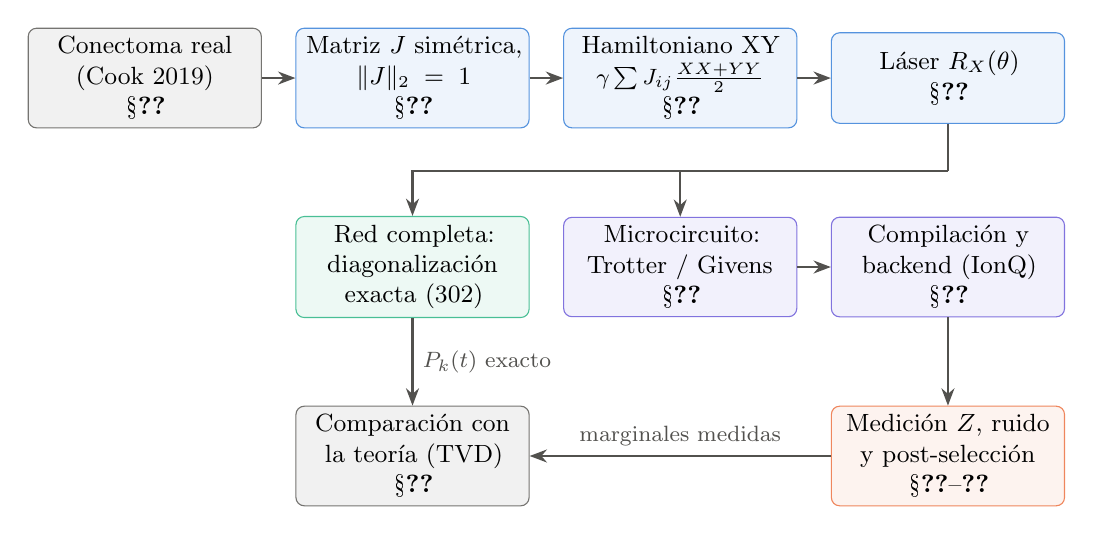
\begin{tikzpicture}[
  caja/.style={draw=#1!80,fill=#1!8,rounded corners=3pt,align=center,font=\small,
               minimum height=1.15cm,text width=2.75cm,inner sep=3pt},
  flecha/.style={-{Stealth[length=2.2mm]},thick,draw=tinta}]
\node[caja=tinta]   (datos)  at (0,0)    {Conectoma real\\ (Cook 2019)\\ \S\ref{sec:conectoma}};
\node[caja=azul]    (J)      at (3.4,0)  {Matriz $J$ simétrica,\\ $\lVert J\rVert_2=1$\\ \S\ref{sec:conectoma}};
\node[caja=azul]    (H)      at (6.8,0)  {Hamiltoniano XY\\ {\footnotesize$\gamma\sum J_{ij}\frac{XX+YY}{2}$}\\ \S\ref{sec:xy}};
\node[caja=azul]    (laser)  at (10.2,0) {Láser $\RX(\theta)$\\ \S\ref{sec:laser}};
\node[caja=verde]   (exacto) at (3.4,-2.4) {Red completa:\\ diagonalización\\ exacta (302)};
\node[caja=violeta] (circ)   at (6.8,-2.4) {Microcircuito:\\ Trotter / Givens\\ \S\ref{sec:circuito}};
\node[caja=violeta] (hw)     at (10.2,-2.4) {Compilación y\\ backend (IonQ)\\ \S\ref{sec:compilacion}};
\node[caja=tinta]   (comp)   at (3.4,-4.8) {Comparación con\\ la teoría (TVD)\\ \S\ref{sec:medicion}};
\node[caja=naranjo] (med)    at (10.2,-4.8) {Medición $Z$, ruido\\ y post-selección\\ \S\ref{sec:ruido}--\ref{sec:mitigacion}};
\draw[flecha] (datos) -- (J);
\draw[flecha] (J) -- (H);
\draw[flecha] (H) -- (laser);
\draw[thick,draw=tinta] (laser.south) -- ++(0,-0.6) coordinate (bus);
\draw[flecha] (bus) -| (exacto.north);
\draw[flecha] (bus -| circ.north) -- (circ.north);
\draw[flecha] (circ) -- (hw);
\draw[flecha] (hw) -- (med);
\draw[flecha] (med) -- node[above,font=\footnotesize,text=tinta]{marginales medidas} (comp);
\draw[flecha] (exacto) -- node[right,font=\footnotesize,text=tinta]{$P_k(t)$ exacto} (comp);
\end{tikzpicture}
\caption{Mapa del modelo. La rama verde es la animación 3D de la red completa; la violeta, el experimento en qubits.}
\label{fig:mapa}
\end{figure}

\subsection{Qué es y qué no es}

\begin{honestidad}
\textbf{Esto no es un modelo biofísico.} Las neuronas reales son sistemas clásicos y disipativos, con potenciales de membrana y canales iónicos en escalas de milisegundos. Aquí \emph{no} se afirma que el cerebro sea cuántico. La analogía es \emph{estructural}: el conectoma real es la ``pista'' por la que viaja una excitación cuántica, y la optogenética inspira cómo se inyecta esa excitación.

\textbf{Con un solo láser no hay ventaja cuántica.} La dinámica queda en un subespacio de dimensión $n$ (\cref{sec:xy}), que el computador clásico resuelve en tiempo polinomial; así se calculan las 302 neuronas. El hardware no ``gana'': \emph{demuestra} la física y permite medir cuánto la degradan el error algorítmico y el ruido. El régimen clásicamente difícil aparece con varios láseres simultáneos (\cref{subsec:varios-laseres,sec:extensiones}).
\end{honestidad}

% =====================================================================
\section{Del conectoma a una matriz hermítica}
\label{sec:conectoma}
% =====================================================================

\subsection{Datos}

\begin{itemize}
\item \textbf{Sinapsis.} Se usan las sinapsis químicas y las uniones gap (eléctricas) del hermafrodita adulto de Cook \emph{et al.}~\cite{cook2019}, en la versión que distribuye OpenWorm~\cite{openworm}. Para cada par de neuronas $(i,j)$ se tiene el número $c_{i\to j}$ de sinapsis químicas de $i$ a $j$ y el número $g_{ij}$ de contactos gap.
\item \textbf{Posiciones y tipos.} La posición 3D de cada soma y su clase (sensorial, interneurona o motora) vienen de OpenWorm CElegansNeuroML. El eje anteroposterior va de unos $-312$ a $410\,\mu$m. Las posiciones \emph{solo} se usan para dibujar; no entran en la física.
\end{itemize}

\subsection{Simetrización: por qué y cómo}

Un hamiltoniano debe ser hermítico ($H=H^\dagger$) para que la evolución $\e^{-\ii Ht}$ sea unitaria, es decir, para que la probabilidad total se conserve. Con coeficientes reales, eso exige una matriz de acoplamientos \emph{simétrica}. Las sinapsis químicas tienen dirección, así que se simetrizan:
\begin{equation}
n_{ij} \;=\; c_{i\to j} + c_{j\to i} + \max(g_{ij},g_{ji}),
\qquad
W_{ij} \;=\; \log\!\left(1+n_{ij}\right),
\qquad W_{ii}=0 .
\label{eq:pesos}
\end{equation}

El máximo en el término gap evita contar dos veces un mismo contacto eléctrico que aparezca listado en ambos sentidos. El logaritmo comprime la cola pesada de la distribución de conteos: unas pocas conexiones con decenas de sinapsis no deben dominar toda la dinámica. Con $\log(1+n)$, el peso crece con $n$ pero cada sinapsis adicional aporta cada vez menos.

\begin{honestidad}
Al simetrizar se \emph{pierde} la dirección de la sinapsis química: en el modelo la excitación puede ir de $j$ a $i$ aunque biológicamente la señal solo vaya de $i$ a $j$. En la \cref{sec:extensiones} se discuten dos formas de recuperarla, ninguna de ellas gratuita.
\end{honestidad}

\subsection{Normalización espectral}

\begin{equation}
J \;=\; \frac{W}{\lambda_{\max}(W)} .
\label{eq:normalizacion}
\end{equation}

\begin{proposicion}\label{prop:norma}
$\lVert J\rVert_2 = 1$. Es decir, el mayor valor propio de $J$ es $1$ y todos los demás cumplen $|\lambda|\le 1$.
\end{proposicion}

\begin{proof}
$W$ es real, simétrica y con entradas no negativas. Por ser simétrica, sus valores propios son reales y $\lVert W\rVert_2=\max_m|\lambda_m|=\rho(W)$, el radio espectral. Por el teorema de Perron--Frobenius para matrices no negativas, $\rho(W)$ es valor propio de $W$; como es el mayor en módulo, coincide con $\lambda_{\max}(W)$. Dividiendo por esa cantidad, $\rho(J)=1=\lambda_{\max}(J)$.
\end{proof}

Con los datos reales se obtiene $\lambda_{\max}(W)\approx 60.2$, y el espectro de $J$ queda en $[-0.40,\,1]$. Hay $3\,465$ pares de neuronas conectados, con $J_{ij}\in[0.012,\,0.073]$.

\paragraph{Unidades de tiempo.} El hamiltoniano será $\gamma J$ (\cref{sec:xy}). Como $\lVert J\rVert_2=1$, la escala de energía más rápida de la red es $\gamma$ y el tiempo se mide en unidades de $1/\gamma$. Un acoplamiento típico $J_{ij}\sim0.04$ tarda del orden de $t\sim 1/(\gamma J_{ij})\approx 25/\gamma$ en transferir una excitación entre dos neuronas aisladas. Por eso los tiempos de la interfaz van de $10$ a $200$.

\subsection{Microcircuitos: restringir la red}
\label{subsec:microcircuitos}

Para el hardware se toma un subconjunto $S$ de neuronas (por ejemplo el circuito de toque~\cite{chalfie1985} \code{toque-6} = \{AVM, ALML, AVDL, AVAL, PVCL, PLML\}) y se usa la \emph{misma} escala global:
\begin{equation}
J_S \;=\; J[S,S].
\end{equation}

Es decir, el hamiltoniano del microcircuito es literalmente la restricción del de la red completa a los qubits de $S$. Con ello el microcircuito queda \emph{aislado}: se ignoran sus acoplamientos con las otras neuronas. Para cuantificar qué se pierde, se escribe $J$ en bloques $S$ y $\bar S$ (el resto) y se expande:
\begin{equation}
\bigl[\e^{-\ii\gamma Jt}\bigr]_{SS}
= \mathbb 1 - \ii\gamma t\,J_{SS} - \tfrac{(\gamma t)^2}{2}\bigl(J_{SS}^2 + J_{S\bar S}J_{\bar S S}\bigr) + O(t^3),
\qquad
\e^{-\ii\gamma J_S t} = \mathbb 1 - \ii\gamma t\,J_{SS} - \tfrac{(\gamma t)^2}{2}J_{SS}^2 + O(t^3).
\end{equation}

Ambas evoluciones coinciden a primer orden y difieren desde el segundo, en el término $J_{S\bar S}J_{\bar SS}$. Ese término describe la excitación que sale de $S$ hacia el resto y vuelve. Para tiempos largos la diferencia es grande. El microcircuito es entonces un modelo del \emph{circuito de toque por sí solo}, igual que en los experimentos que lo estudian aislado, y no una ventana a la red completa.

% =====================================================================
\section{El hamiltoniano XY y el quantum walk}
\label{sec:xy}
% =====================================================================

\subsection{Definición}

Se asigna un qubit a cada neurona: $\ket{0}$ es reposo y $\ket{1}$ es excitación. Con las matrices de Pauli $X,Y,Z$ (\cref{app:pauli}) y $Z\ket{0}=\ket{0}$, $Z\ket{1}=-\ket{1}$, los operadores de subida y bajada son
\begin{equation}
\sigma^+ \equiv \ket{1}\!\bra{0} = \tfrac12(X-\ii Y),
\qquad
\sigma^- \equiv \ket{0}\!\bra{1} = \tfrac12(X+\ii Y).
\label{eq:sigmas}
\end{equation}

\begin{definicion}[Hamiltoniano XY sobre el conectoma]
\begin{equation}
H \;=\; \gamma\sum_{i<j} J_{ij}\,\frac{X_iX_j+Y_iY_j}{2}
\;=\; \gamma\sum_{i<j} J_{ij}\,\bigl(\sigma_i^+\sigma_j^- + \sigma_i^-\sigma_j^+\bigr).
\label{eq:HXY}
\end{equation}
\end{definicion}

\begin{proof}[Verificación de la igualdad]
Con \eqref{eq:sigmas},
\begin{align*}
\sigma_i^+\sigma_j^- + \sigma_i^-\sigma_j^+
&= \tfrac14\bigl[(X_i-\ii Y_i)(X_j+\ii Y_j) + (X_i+\ii Y_i)(X_j-\ii Y_j)\bigr]\\
&= \tfrac14\bigl[2X_iX_j + 2Y_iY_j + \ii(X_iY_j - Y_iX_j) - \ii(X_iY_j - Y_iX_j)\bigr]
= \tfrac12\,(X_iX_j+Y_iY_j). \qedhere
\end{align*}
\end{proof}

La segunda forma de \eqref{eq:HXY} muestra que cada término \emph{mueve} una excitación: $\sigma_i^+\sigma_j^-$ la quita de $j$ y la pone en $i$, con amplitud $\gamma J_{ij}$. Es el modelo XY, también llamado de \emph{bosones de núcleo duro} (\emph{hard-core bosons}): partículas que saltan por el grafo sin poder ocupar dos a la vez el mismo sitio, porque un qubit solo admite una excitación.

\subsection{Tres propiedades clave}

\begin{proposicion}[Conservación del número de excitaciones]\label{prop:conservacion}
Sea $\Nop=\sum_k \sigma_k^+\sigma_k^- = \sum_k \tfrac12(\mathbb 1 - Z_k)$, que cuenta los qubits en $\ket1$. Entonces $[H,\Nop]=0$.
\end{proposicion}

\begin{proof}
Para un qubit, $\Nop_k\sigma_k^+ = \proj1\,\ket1\!\bra0 = \sigma_k^+$ y $\sigma_k^+\Nop_k = \ket1\!\bra0\,\proj1 = 0$. Luego $[\Nop_k,\sigma_k^+] = \sigma_k^+$ y, de la misma forma, $[\Nop_k,\sigma_k^-]=-\sigma_k^-$. Como operadores sobre qubits distintos conmutan, para $i\ne j$
\[
[\Nop,\sigma_i^+\sigma_j^-] = [\Nop_i,\sigma_i^+]\,\sigma_j^- + \sigma_i^+[\Nop_j,\sigma_j^-] = \sigma_i^+\sigma_j^- - \sigma_i^+\sigma_j^- = 0,
\]
y lo mismo para el término conjugado. Sumando sobre los pares, $[\Nop,H]=0$.
\end{proof}

En consecuencia, $H$ es diagonal por bloques en los \emph{sectores} de $k$ excitaciones, de dimensión $\binom{n}{k}$, y la dinámica nunca mezcla sectores distintos. Esta ley de conservación es la base de la mitigación de la \cref{sec:mitigacion}.

\begin{proposicion}[El vacío es estacionario]\label{prop:vacio}
Si $\vac=\ket{0\cdots0}$, entonces $H\vac=0$ y $\e^{-\ii Ht}\vac=\vac$ para todo $t$.
\end{proposicion}

\begin{proof}
$\sigma_j^-\ket0=0$, así que cada término de \eqref{eq:HXY} aniquila $\vac$.
\end{proof}

\begin{proposicion}[Sector de una excitación = quantum walk]\label{prop:ctqw}
Sea $\ket{e_k}=\sigma_k^+\vac$ el estado con solo la neurona $k$ excitada. Entonces
\begin{equation}
H\ket{e_k} = \gamma\sum_i J_{ik}\ket{e_i}
\qquad\Longrightarrow\qquad
\bra{e_i}\e^{-\ii Ht}\ket{e_j} = \bigl[\e^{-\ii\gamma Jt}\bigr]_{ij}.
\label{eq:ctqw}
\end{equation}
\end{proposicion}

\begin{proof}
Para $i\neq j$, $\sigma_i^+\sigma_j^-\ket{e_k}$ es distinto de cero solo si $j=k$ (hay que bajar la neurona excitada) y $i\ne k$; en ese caso vale $\ket{e_i}$. Así, $\sigma_i^+\sigma_j^-\ket{e_k}=\delta_{jk}\ket{e_i}$. Sumando ambos términos del hamiltoniano y usando $J_{ik}=J_{ki}$ y $J_{kk}=0$, se obtiene $H\ket{e_k}=\gamma\sum_i J_{ik}\ket{e_i}$. En la base $\{\ket{e_k}\}$, la restricción de $H$ al sector de una excitación es entonces la matriz $\gamma J$. Como el sector es invariante (\cref{prop:conservacion}), la exponencial de $H$ restringida es la exponencial de $\gamma J$.
\end{proof}

La \cref{prop:ctqw} dice que, en este sector, el modelo XY es \emph{exactamente} el \emph{quantum walk de tiempo continuo} (CTQW) de Farhi y Gutmann~\cite{farhi1998} con hamiltoniano $\gamma J$; ver~\cite{childs2009,mulken2011} para su papel en computación y en transporte sobre redes complejas. Una excitación en un sistema de $n$ qubits ($2^n$ amplitudes) se describe así con un vector de solo $n$ amplitudes.

\subsection{Cálculo exacto en la red completa}

$J$ es real y simétrica, así que $J=V\Lambda V^{\top}$ con $V$ ortogonal y $\Lambda=\mathrm{diag}(\lambda_1,\dots,\lambda_n)$. Entonces
\begin{equation}
\bigl[\e^{-\ii\gamma Jt}\bigr]_{kj} = \sum_{m=1}^{n} V_{km}\,\e^{-\ii\gamma\lambda_m t}\,V_{jm}.
\label{eq:espectral}
\end{equation}

Se diagonaliza una sola vez, con costo $O(n^3)$, y luego cada instante cuesta $O(n^2)$. Para $n=302$ y 160 fotogramas son milisegundos. Esto es lo que hace \code{fisica.probabilidades\_walk}.

\subsection{Cómo se ve un quantum walk}
\label{subsec:como-se-ve}

\paragraph{Ballístico frente a difusivo.} El contraste más limpio aparece en una cadena: un camino de $n$ sitios con $J_{x,x+1}=1$. El análogo clásico es la difusión $\dot{\bm p}=-\gamma L\bm p$, donde $L=D-J$ es el laplaciano del grafo y $D$ la matriz diagonal de grados. En una cadena infinita la amplitud cuántica es $\bk{x}{\psi(t)}=(-\ii)^{|x|}\,\mathcal J_x(2\gamma t)$ (función de Bessel), y usando $\sum_x x^2\mathcal J_x(z)^2=z^2/2$ se obtiene
\begin{equation}
\sigma_{\text{cuántico}}(t)=\sqrt2\,\gamma t,
\qquad
\sigma_{\text{clásico}}(t)=\sqrt{2\gamma t}.
\end{equation}

La excitación cuántica se dispersa en forma \emph{lineal} con el tiempo, la clásica como $\sqrt t$, y el perfil cuántico muestra franjas de interferencia (\cref{fig:cadena}).

\begin{figure}[htbp]
\centering
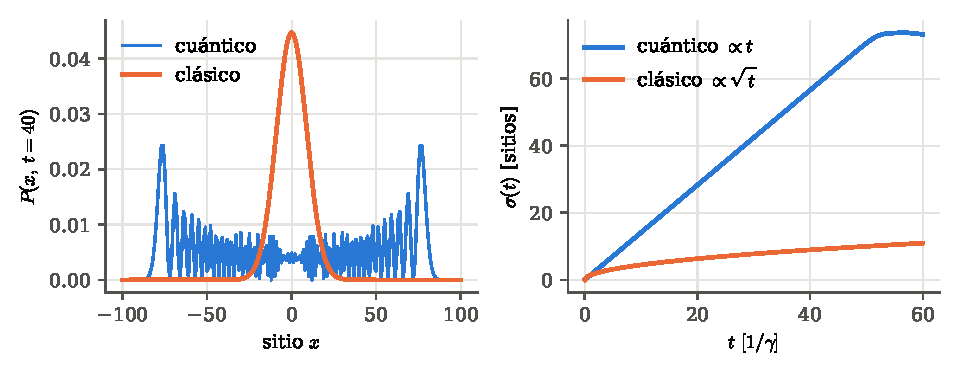
\includegraphics[width=\textwidth]{figuras/fig_cadena.pdf}
\caption{Cadena de 201 sitios, excitación inicial en el centro. Izquierda: distribución en $t=40$; el frente cuántico avanza a velocidad constante y deja franjas de interferencia. Derecha: dispersión $\sigma(t)$. La curva cuántica sigue $\sqrt2\,t$ hasta que el frente choca con el borde ($t\approx50$).}
\label{fig:cadena}
\end{figure}

\paragraph{En el conectoma.} El conectoma es un grafo de mundo pequeño: casi cualquier par de neuronas está a dos o tres sinapsis de distancia. Ahí la difusión clásica llega muy rápido a su estado estacionario, la distribución uniforme, de modo que la ventaja ``balística'' no se nota. La diferencia importante es otra (\cref{fig:conectoma}):

\begin{itemize}
\item \textbf{El walk cuántico no converge.} Como la evolución es unitaria, no hay estado estacionario. Lo que sí existe es el promedio temporal
\begin{equation}
\overline{P_k} = \lim_{T\to\infty}\frac1T\int_0^T P_k(t)\,dt
= \sum_{\lambda}\Bigl|\sum_{m:\,\lambda_m=\lambda} V_{km}V_{jm}\Bigr|^2,
\end{equation}
que depende de la neurona inicial $j$: el walk \emph{recuerda} dónde empezó.
\item \textbf{Interferencia.} Neuronas cercanas pueden quedar casi apagadas, porque las amplitudes de distintos caminos se cancelan, mientras que neuronas más lejanas se encienden.
\end{itemize}

Una forma de medir cuán repartida está la excitación es la \emph{participación efectiva}
\begin{equation}
\mathrm{PR}(t) = \frac{1}{\sum_k q_k(t)^2},\qquad q_k = \frac{P_k}{\sum_l P_l},
\end{equation}
que vale $1$ si la excitación está en una sola neurona y $n$ si está repartida por igual. Desde AVM, en $t=60$ el walk cuántico tiene $\mathrm{PR}\approx130$, mientras que la difusión clásica ya llegó a $\approx283$, casi uniforme.

\begin{figure}[htbp]
\centering
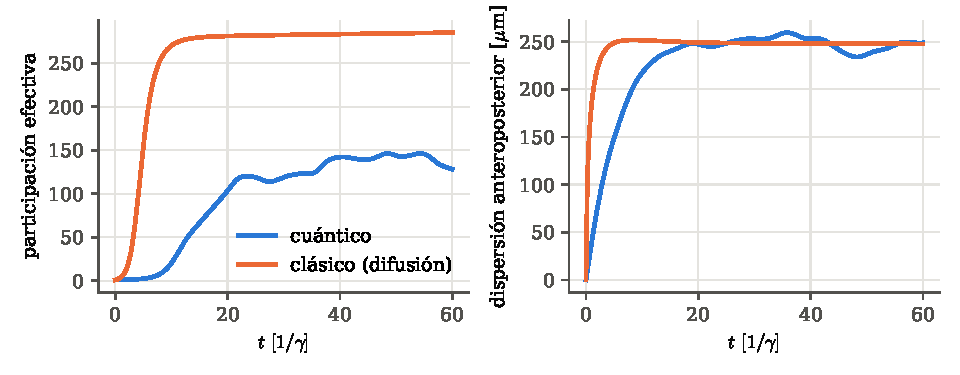
\includegraphics[width=\textwidth]{figuras/fig_walk_vs_clasico.pdf}
\caption{Conectoma completo, láser en AVM. Izquierda: participación efectiva. Derecha: dispersión del centro de masa a lo largo del eje anteroposterior. La difusión clásica se uniformiza en $t\approx10$; el walk cuántico sigue fluctuando y se mantiene más concentrado.}
\label{fig:conectoma}
\end{figure}

\begin{observacion}[Por qué no basta con fermiones libres]
En una cadena unidimensional, la transformación de Jordan--Wigner convierte el modelo XY en fermiones \emph{libres}, que se resuelven con $n\times n$ matrices para cualquier número de excitaciones. En un grafo general como el conectoma, las ``cuerdas'' de Jordan--Wigner no se cancelan y aparecen interacciones: con dos o más excitaciones el problema es genuinamente de muchos cuerpos. Con una excitación esto no importa, porque la \cref{prop:ctqw} ya es exacta.
\end{observacion}

% =====================================================================
\section{El láser optogenético como rotación de Rabi}
\label{sec:laser}
% =====================================================================

\subsection{De un pulso de luz a $\RX(\theta)$}

Se modela la neurona iluminada como un sistema de dos niveles excitado por un campo casi resonante. En el marco que rota con el campo, y con la aproximación de onda rotante, el hamiltoniano de control es
\begin{equation}
H_{\text{pulso}} = \frac{\Delta}{2}Z + \frac{\Omega}{2}\bigl(\cos\varphi\,X + \sin\varphi\,Y\bigr),
\end{equation}
donde $\Omega$ es la frecuencia de Rabi (proporcional a la amplitud del campo), $\Delta$ la desintonía y $\varphi$ la fase del pulso; el signo de $\Delta$ depende de la convención del marco. En resonancia ($\Delta=0$) y con $\varphi=0$, un pulso de duración $\tau$ produce
\begin{equation}
U = \e^{-\ii\Omega\tau X/2} = \RX(\theta),\qquad \theta=\Omega\tau,
\qquad
\RX(\theta)\ket0 = \cos\tfrac\theta2\ket0 - \ii\sin\tfrac\theta2\ket1 .
\end{equation}

La probabilidad de excitar la neurona es $\sin^2(\theta/2)$: con $\theta=\pi$ (pulso $\pi$) el disparo es seguro, y con $\theta=\pi/2$ ocurre la mitad de las veces. Fuera de resonancia vale la fórmula de Rabi, $P=\frac{\Omega^2}{\Omega^2+\Delta^2}\sin^2\!\bigl(\tfrac12\sqrt{\Omega^2+\Delta^2}\,\tau\bigr)$, que nunca llega a $1$; el modelo usa el caso resonante.

\paragraph{Aproximación de pulso corto.} Se supone que el pulso dura mucho menos que la dinámica de la red, $\tau\ll1/\gamma$. Así la red no evoluciona mientras se ilumina y la operación completa es
\begin{equation}
\ket{\psi(t)} = \e^{-\ii Ht}\,\RX^{(j)}(\theta)\,\vac .
\end{equation}

\subsection{El resultado central}

\begin{proposicion}[Probabilidad de disparo]\label{prop:central}
Si se ilumina la neurona $j$ con un pulso $\theta$ y la red empieza en reposo, entonces
\begin{equation}
\ket{\psi(t)} = \cos\tfrac\theta2\,\vac \;-\;\ii\sin\tfrac\theta2\sum_k\bigl[\e^{-\ii\gamma Jt}\bigr]_{kj}\ket{e_k},
\end{equation}
y la probabilidad de que la neurona $k$ se mida en $\ket1$ es
\begin{equation}
\boxed{\;P_k(t) = \sin^2\!\frac\theta2\;\Bigl|\bigl[\e^{-\ii\gamma Jt}\bigr]_{kj}\Bigr|^2\;}
\label{eq:central}
\end{equation}
Además, $\sum_kP_k(t)=\sin^2(\theta/2)$ y la probabilidad de no medir ninguna excitación es $\cos^2(\theta/2)$, constante en el tiempo.
\end{proposicion}

\begin{proof}
$\RX^{(j)}(\theta)\vac = \cos\frac\theta2\vac - \ii\sin\frac\theta2\ket{e_j}$. Por linealidad, el primer término no evoluciona (\cref{prop:vacio}) y el segundo evoluciona con la \cref{prop:ctqw}. Como los $\ket{e_k}$ y $\vac$ son estados de la base computacional, ortogonales entre sí, la probabilidad de medir $\ket1$ en el qubit $k$ es el módulo al cuadrado del coeficiente de $\ket{e_k}$. La suma sobre $k$ es $\sin^2\frac\theta2\,\lVert\e^{-\ii\gamma Jt}\bm e_j\rVert^2=\sin^2\frac\theta2$, porque la evolución es unitaria.
\end{proof}

\begin{idea}[Cómo leer la fórmula]
La intensidad del láser ($\theta$) solo escala el \emph{tamaño} de la respuesta. El \emph{patrón} de propagación, es decir qué neuronas se encienden y cuándo, lo fija únicamente el conectoma a través de $\e^{-\ii\gamma Jt}$. Esta fórmula es exactamente lo que dibuja la animación 3D.
\end{idea}

\begin{observacion}[La coherencia con el vacío]
El estado es una superposición coherente entre ``no pasó nada'' y ``hay una excitación viajando''. Medir en base $Z$ no ve esa coherencia, porque las probabilidades no dependen de la fase relativa. Una medición en otra base, por ejemplo $X$ en un qubit, sí la vería: es una extensión natural (\cref{sec:extensiones}).
\end{observacion}

\subsection{Varios láseres}
\label{subsec:varios-laseres}

Si se ilumina un conjunto $S$ de neuronas con el mismo $\theta$,
\begin{equation}
\bigotimes_{s\in S}\RX^{(s)}(\theta)\,\vac
= \sum_{A\subseteq S}\Bigl(\cos\tfrac\theta2\Bigr)^{|S|-|A|}\Bigl(-\ii\sin\tfrac\theta2\Bigr)^{|A|}\ket{e_A},
\end{equation}
donde $\ket{e_A}$ tiene excitadas exactamente las neuronas de $A$. El estado ocupa los sectores $0,\dots,|S|$ con pesos binomiales. En el sector de $k\ge2$ excitaciones, la dinámica \emph{no} se reduce a $J$: la regla de núcleo duro (dos excitaciones no pueden estar en la misma neurona) actúa como una interacción. La dimensión del sector es $\binom nk$; para $n=302$ son $45\,451$ estados con $k=2$ y $4\,545\,100$ con $k=3$. Ahí la simulación clásica crece combinatoriamente y la simulación cuántica tiene sentido real.

% =====================================================================
\section{Medición: \emph{spikes}, marginales y distancias}
\label{sec:medicion}
% =====================================================================

\subsection{Qué se mide}

Cada ejecución del circuito (un \emph{shot}) mide todos los qubits en base $Z$ y devuelve una cadena de bits $b=(b_0,\dots,b_{n-1})$: el patrón de activación del microcircuito, donde $b_k=1$ significa que la neurona $k$ disparó. Por la regla de Born, la cadena $b$ aparece con probabilidad $p(b)=|\bk{b}{\psi}|^2$. La probabilidad de disparo de la neurona $k$ es la \emph{marginal}
\begin{equation}
P_k = \sum_{b:\,b_k=1} p(b).
\end{equation}

\paragraph{Orden de los bits en Qiskit.} Qiskit escribe las cadenas con el qubit $0$ a la \emph{derecha}: la clave \code{'000010'} significa que $q_1$ está en $\ket1$. El código convierte cada clave con \code{int(clave, 2)}, que da exactamente el índice cuyo bit menos significativo es $q_0$ (\code{analisis.conteos\_a\_probs}).

\paragraph{Error estadístico.} Con $S$ shots, la marginal estimada $\hat P_k$ es una proporción binomial:
\begin{equation}
\operatorname{desv}(\hat P_k)=\sqrt{\frac{P_k(1-P_k)}{S}}\;\le\;\frac{1}{2\sqrt S}.
\end{equation}

Con $S=500$ la incertidumbre es como mucho $0.022$; para bajarla a la mitad hay que cuadruplicar los shots.

\subsection{Distancia de variación total}

Para comparar dos distribuciones $p,q$ sobre las $2^n$ cadenas se usa
\begin{equation}
\TVD(p,q) = \frac12\sum_b|p(b)-q(b)| = \max_{E}\,|p(E)-q(E)|,
\end{equation}
la mayor diferencia de probabilidad que las distribuciones asignan a un mismo evento $E$. Vale $0$ si son iguales y $1$ si no se solapan. Como cada marginal es la probabilidad de un evento ($b_k=1$), se cumple
\begin{equation}
|P_k - Q_k|\le\TVD(p,q)\qquad\text{para toda neurona }k.
\end{equation}

Además, por la desigualdad triangular,
\begin{equation}
\TVD(p_{\text{exacta}},p_{\text{medida}}) \le
\underbrace{\TVD(p_{\text{exacta}},p_{\text{circuito ideal}})}_{\text{error algorítmico}}
+ \underbrace{\TVD(p_{\text{circuito ideal}},p_{\text{medida}})}_{\text{ruido + muestreo}},
\label{eq:triangular}
\end{equation}
que permite separar las fuentes de error. Incluso un backend perfecto tiene un piso de error por muestreo: con pocos shots, la TVD entre la distribución empírica y la verdadera no es cero. Por eso un simulador ideal con 500 shots da TVD algo mayor que la del circuito exacto.

% =====================================================================
\section{Del hamiltoniano al circuito}
\label{sec:circuito}
% =====================================================================

\subsection{La compuerta de salto}

Para una sinapsis $e=(a,b)$ se define el término $h_e = \gamma J_{ab}(X_aX_b+Y_aY_b)/2$, de modo que $H=\sum_e h_e$.

\begin{lema}\label{lema:hop}
$X_aX_b$ y $Y_aY_b$ conmutan. Por lo tanto, con la convención de Qiskit $R_{PP}(\alpha)=\e^{-\ii\alpha PP/2}$,
\begin{equation}
\hop(\alpha)\equiv\e^{-\ii\alpha(XX+YY)/2} = \RXX(\alpha)\,\RYY(\alpha),
\qquad
\e^{-\ii h_e\delta} = \hop(\gamma J_{ab}\delta).
\end{equation}
\end{lema}

\begin{proof}
En cada qubit, $XY=-YX$. Al pasar $X_aX_b$ a través de $Y_aY_b$ aparecen dos signos $-1$, uno por qubit, y se cancelan: $X_aX_bY_aY_b=Y_aY_bX_aX_b$. Para operadores que conmutan, $\e^{A+B}=\e^A\e^B$.
\end{proof}

En la base $\{\ket{00},\ket{01},\ket{10},\ket{11}\}$, como $XX\ket{00}=\ket{11}$ y $YY\ket{00}=-\ket{11}$, se tiene $(XX+YY)\ket{00}=0$, e igual para $\ket{11}$. En cambio, $(XX+YY)/2$ intercambia $\ket{01}\leftrightarrow\ket{10}$. Luego
\begin{equation}
\hop(\alpha)=
\begin{pmatrix}
1&0&0&0\\
0&\cos\alpha&-\ii\sin\alpha&0\\
0&-\ii\sin\alpha&\cos\alpha&0\\
0&0&0&1
\end{pmatrix}.
\label{eq:hopmatriz}
\end{equation}

La compuerta deja quietos $\ket{00}$ y $\ket{11}$, y rota una excitación entre las dos neuronas un ángulo $\alpha$. Es una rotación de Givens en el sector de una excitación~\cite{kivlichan2018}, y conserva $\Nop$ igual que $H$.

\subsection{Trotter--Suzuki (modo \code{trotter})}

Los términos $h_e$ no conmutan entre sí cuando comparten una neurona, así que $\e^{-\ii Ht}\ne\prod_e\e^{-\ii h_et}$. La fórmula de Lie--Trotter divide el tiempo en $r$ pasos de duración $\delta=t/r$:
\begin{align}
U_1(\delta) &= \prod_{e=1}^{|E|}\e^{-\ii h_e\delta}
&&\text{(1.\textsuperscript{er} orden)},\\
U_2(\delta) &= \prod_{e=1}^{|E|}\e^{-\ii h_e\delta/2}\;\prod_{e=|E|}^{1}\e^{-\ii h_e\delta/2}
&&\text{(2.\textsuperscript{o} orden, Strang)},
\end{align}
y aproxima $\e^{-\ii Ht}\approx U(\delta)^r$.

\begin{proposicion}[Error de Trotter]\label{prop:trotter}
\begin{equation}
\bigl\lVert\e^{-\ii Ht}-U_1(t/r)^r\bigr\rVert\le\frac{t^2}{2r}\sum_{a<b}\bigl\lVert[h_a,h_b]\bigr\rVert,
\qquad
\bigl\lVert\e^{-\ii Ht}-U_2(t/r)^r\bigr\rVert=O\!\left(\frac{t^3}{r^2}\right).
\end{equation}
\end{proposicion}

\begin{proof}[Idea de la demostración]
Para dos términos, la fórmula de Baker--Campbell--Hausdorff da
\[
\e^{-\ii A\delta}\e^{-\ii B\delta}=\exp\Bigl(-\ii(A+B)\delta-\tfrac{\delta^2}{2}[A,B]+O(\delta^3)\Bigr).
\]
Cada paso comete entonces un error de orden $\frac{\delta^2}2\lVert[A,B]\rVert$; con más términos aparecen todos los pares, $\frac{\delta^2}{2}\sum_{a<b}\lVert[h_a,h_b]\rVert$. Como los operadores son unitarios, los errores de los $r$ pasos se suman a lo más linealmente: $r\cdot\frac{(t/r)^2}2\sum\lVert[h_a,h_b]\rVert$. En la fórmula simétrica de Strang, el término de orden $\delta^2$ se cancela (el producto es invariante bajo $\delta\to-\delta$ e inversión), así que el error por paso es $O(\delta^3)$ y el total $O(t^3/r^2)$. Las cotas finas, que dependen solo de conmutadores, están en~\cite{childs2021}.
\end{proof}

\paragraph{Qué conmutadores importan.} $[h_a,h_b]=0$ si las sinapsis $a$ y $b$ no comparten neurona, porque actúan sobre qubits distintos. El error de Trotter depende entonces de la estructura \emph{local} del grafo, es decir de cuántas sinapsis inciden en cada neurona, y no del tamaño total de la red.

\paragraph{Fusión de saltos.} Dos mitades consecutivas sobre el mismo par se pueden juntar exactamente, porque un término conmuta consigo mismo: $\hop(\alpha)\hop(\beta)=\hop(\alpha+\beta)$. Dentro de cada paso de Strang se fusiona el centro (el último salto del producto directo con el primero del inverso). Entre pasos se fusionan el último salto de un paso y el primero del siguiente. Un circuito de $r$ pasos de 2.\textsuperscript{o} orden queda con
\begin{equation}
N_{\hop}=r\,(2|E|-1)-(r-1)=(2|E|-2)\,r+1
\end{equation}
saltos, cada uno de 2 compuertas de dos qubits ($\RXX$ y $\RYY$). Para \code{toque-6} ($|E|=8$, $r=2$) son $29$ saltos y $58$ compuertas de dos qubits.

\begin{figure}[htbp]
\centering
\begin{quantikz}[row sep=0.25cm, column sep=0.3cm]
\lstick{$q_0$: AVM}  & \gate{\RX(\theta)} & \gate[2]{\hop\!\left(\tfrac{\alpha_{01}}{2}\right)} & \qw & \gate[2]{\hop\!\left(\tfrac{\alpha_{01}}{2}\right)} & \meter{}\\
\lstick{$q_1$: ALML} & \qw & & \gate[2]{\hop(\alpha_{12})} & & \meter{}\\
\lstick{$q_2$: AVDL} & \qw & \qw & & \qw & \meter{}
\end{quantikz}
\\[10pt]
\begin{quantikz}[row sep=0.25cm, column sep=0.3cm]
& \gate[2]{\hop(\alpha)} & \qw \\
& & \qw
\end{quantikz}
=
\begin{quantikz}[row sep=0.25cm, column sep=0.3cm]
& \gate[2]{\RXX(\alpha)} & \gate[2]{\RYY(\alpha)} & \qw\\
& & & \qw
\end{quantikz}
\caption{Arriba: un paso de Strang para una cadena de tres neuronas (sinapsis $0$--$1$ y $1$--$2$), con $\alpha_{ab}=\gamma J_{ab}\,\delta$; el salto central $1$--$2$ ya está fusionado. Abajo: cada salto son dos compuertas estándar de Qiskit.}
\label{fig:circuito}
\end{figure}

En Qiskit, el circuito se arma así (\code{circuitos.a\_qiskit}):

\begin{lstlisting}
qc = QuantumCircuit(n, n)
qc.rx(theta, fuente)                 # laser optogenetico
for (a, b, alfa) in saltos:          # Trotter o Givens
    qc.rxx(alfa, a, b)               # exp(-i alfa XX/2)
    qc.ryy(alfa, a, b)               # exp(-i alfa YY/2)
qc.measure(range(n), range(n))
\end{lstlisting}

\Cref{fig:toque6} muestra la teoría exacta del microcircuito \code{toque-6} y lo que da el circuito de Trotter con solo $r=2$ pasos. \Cref{fig:trotter} (izquierda) verifica numéricamente los órdenes de la \cref{prop:trotter}.

\begin{figure}[htbp]
\centering
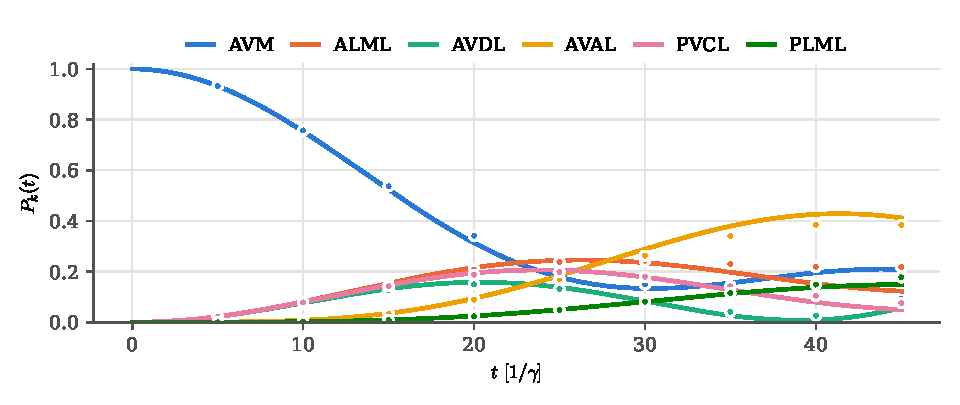
\includegraphics[width=\textwidth]{figuras/fig_toque6.pdf}
\caption{Microcircuito \code{toque-6}, pulso $\theta=\pi$ en AVM, $\gamma=1$. Líneas: teoría exacta $P_k(t)$. Puntos: circuito ideal de Trotter de 2.\textsuperscript{o} orden con $r=2$ pasos para cada $t$. El acuerdo es muy bueno hasta $t\approx15$ y se degrada a tiempos largos, porque con $r$ fijo el paso $\delta=t/r$ crece.}
\label{fig:toque6}
\end{figure}

\begin{figure}[htbp]
\centering
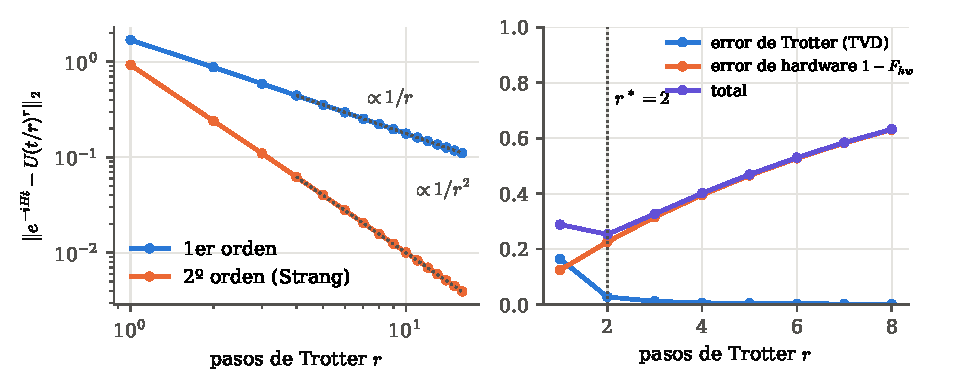
\includegraphics[width=\textwidth]{figuras/fig_trotter.pdf}
\caption{\code{toque-6} en $t=30$. Izquierda: error de operador de Trotter en función del número de pasos; las pendientes confirman $1/r$ y $1/r^2$. Derecha: presupuesto de errores (\cref{sec:ruido}). El error de Trotter (TVD) baja con $r$, el de hardware sube con el número de compuertas, y el total es mínimo en $r^*=2$.}
\label{fig:trotter}
\end{figure}

\paragraph{Las cotas son holgadas.} Para \code{toque-6} en $t=30$ con $r=2$, la cota de 1.\textsuperscript{er} orden de la \cref{prop:trotter} vale $\approx7.1$. El error de operador real es $1.25$ en 1.\textsuperscript{er} orden y $0.49$ en 2.\textsuperscript{o}, y la TVD de la distribución medida es solo $0.093$. La cota sirve para entender cómo escala el error, no para elegir $r$: el código elige $r$ calculando el error de verdad (\cref{sec:ruido}).

\begin{idea}[Por qué este modo es simulación cuántica genuina]
El circuito de Trotter no usa la respuesta: solo usa $J$ y el tiempo. Funciona igual con varios láseres, donde el computador clásico ya no puede seguirlo. Es la idea de Lloyd~\cite{lloyd1996} de un simulador cuántico universal aplicada al conectoma.
\end{idea}

\subsection{Cascada de Givens (modo \code{givens})}
\label{subsec:givens}

Con un láser, el estado final es $\cos\frac\theta2\vac-\ii\sin\frac\theta2\sum_kv_k\ket{e_k}$, con $\bm v=\e^{-\ii\gamma Jt}\bm e_j$, que se calcula clásicamente. Basta entonces con \emph{preparar} un estado cuyas amplitudes tengan los módulos $|v_k|$.

\begin{proposicion}[Preparación con $n-1$ saltos]\label{prop:givens}
Sea $o_0=j,o_1,\dots,o_{n-1}$ un orden de las neuronas que empieza en la iluminada. Se definen $R_0=1$ y, para $m=0,\dots,n-2$,
\begin{equation}
\cos\alpha_m=\frac{|v_{o_m}|}{R_m},\qquad R_{m+1}=R_m\sin\alpha_m .
\end{equation}
Aplicando $\hop(\alpha_m)$ sobre el par $(o_m,o_{m+1})$ en ese orden, después de $\RX^{(j)}(\theta)$, se obtiene un estado cuya distribución en base $Z$ es exactamente la de la \cref{prop:central}.
\end{proposicion}

\begin{proof}
Por \eqref{eq:hopmatriz}, un salto deja $\vac$ intacto y, en el sector de una excitación, lleva $\ket{e_a}\mapsto\cos\alpha\ket{e_a}-\ii\sin\alpha\ket{e_b}$. Por inducción: antes del salto $m$, toda la amplitud que falta repartir, de módulo $R_m$, está en $o_m$. El salto deja en $o_m$ un módulo $R_m\cos\alpha_m=|v_{o_m}|$ y pasa $R_m\sin\alpha_m=R_{m+1}$ a $o_{m+1}$. Como $R_{m+1}^2=R_m^2-|v_{o_m}|^2=1-\sum_{l\le m}|v_{o_l}|^2$, al final $R_{n-1}=|v_{o_{n-1}}|$. Las fases quedan distintas a las de $\bm v$, pero en base $Z$ solo importan los módulos.
\end{proof}

Si las neuronas se ordenan por $|v_k|$ decreciente, $R_m$ cae rápido y los saltos con $\alpha_m\approx0$ se omiten. El modo Givens tiene \emph{profundidad mínima}, $n-1$ saltos frente a los $(2|E|-2)r+1$ de Trotter, y es exacto: en \code{toque-bilateral-10} da $\TVD=0$ con 9 saltos.

\begin{honestidad}
El modo Givens \emph{necesita conocer la respuesta de antemano}, así que no es simulación cuántica. Sirve para validar la lectura del hardware y para mostrar microcircuitos grandes donde Trotter sería demasiado profundo.
\end{honestidad}

% =====================================================================
\section{Compilación y ejecución en hardware}
\label{sec:compilacion}
% =====================================================================

\subsection{Por qué iones atrapados}

\begin{itemize}
\item \textbf{Conectividad total.} En una trampa de iones, cualquier par de qubits puede entrelazarse directamente. El conectoma es un grafo irregular y no planar. En un chip superconductor con conectividad de vecinos cercanos, cada sinapsis entre qubits no adyacentes necesita cadenas de compuertas SWAP (3 CNOT cada una). En IonQ cada sinapsis es una compuerta directa. Qollab permite ver este costo: el mismo circuito transpilado para un simulador con ruido de IBM agrega SWAPs, mientras que en IonQ no.
\item \textbf{Compuerta parametrizada.} IonQ Forte ofrece $ZZ(\theta)$ con ángulo arbitrario, ideal para los saltos pequeños $\gamma J_{ij}\delta$.
\item \textbf{Fidelidades.} Forte tiene 36 qubits, con fidelidades del orden de $99.98\%$ en 1 qubit y $99.6\%$ en 2 qubits~\cite{ionqcompare}.
\end{itemize}

\subsection{Compuertas nativas de IonQ}

IonQ mide las fases en \emph{vueltas} (1 vuelta $=2\pi$)~\cite{ionqnative}:
\begin{equation}
\mathrm{GPi}(\phi)=\begin{pmatrix}0&\e^{-2\pi\ii\phi}\\\e^{2\pi\ii\phi}&0\end{pmatrix},\quad
\mathrm{GPi2}(\phi)=\frac1{\sqrt2}\begin{pmatrix}1&-\ii\e^{-2\pi\ii\phi}\\-\ii\e^{2\pi\ii\phi}&1\end{pmatrix},\quad
ZZ(\theta)=\e^{-\ii\pi\theta\,Z\otimes Z}.
\end{equation}

Reemplazando, $\mathrm{GPi2}(0)=\RX(\pi/2)$ y $\mathrm{GPi2}(\tfrac14)=R_Y(\pi/2)$. Las rotaciones $R_Z$ son \emph{virtuales}: no se aplican como pulso, sino que se absorben en las fases de las compuertas siguientes.

\paragraph{Cada salto cuesta dos $ZZ$.} Rotar $Z$ con $V=R_Y(\pi/2)$ da $VZV^\dagger=X$, y con $W=\RX(\pi/2)$ da $WZW^\dagger=-Y$. Usando $R_Y(\theta)ZR_Y(\theta)^\dagger=\cos\theta\,Z+\sin\theta\,X$ y $\RX(\theta)Z\RX(\theta)^\dagger=\cos\theta\,Z-\sin\theta\,Y$,
\begin{align}
\e^{-\ii\beta XX}&=(V\otimes V)\,ZZ\!\left(\tfrac\beta\pi\right)(V^\dagger\otimes V^\dagger),\\
\e^{-\ii\beta YY}&=(W\otimes W)\,ZZ\!\left(\tfrac\beta\pi\right)(W^\dagger\otimes W^\dagger),
\end{align}
porque $(-Y)\otimes(-Y)=Y\otimes Y$. Con $\beta=\alpha/2$, $\RXX(\alpha)$ y $\RYY(\alpha)$ cuestan una $ZZ(\alpha/2\pi)$ cada una. Dos es además el mínimo: $\hop$ tiene dos coeficientes de Cartan no nulos y una sola $ZZ$ no basta.

\paragraph{El láser.} $\RX(\theta)=\mathrm{GPi2}(\tfrac14)\,R_Z(\theta)\,\mathrm{GPi2}(\tfrac34)$, con la $R_Z$ virtual.

\paragraph{Reducción del ángulo.} Con las identidades exactas
\begin{equation}
ZZ(\theta+1)=-ZZ(\theta),\qquad
ZZ(\theta+\tfrac12)=-\ii\,(Z\otimes Z)\,ZZ(\theta),\qquad
ZZ(-\theta)=(X\otimes\mathbb 1)\,ZZ(\theta)\,(X\otimes\mathbb 1),
\end{equation}
cualquier ángulo se lleva a $[0,\tfrac14]$, que es el rango que el hardware ejecuta con mejor fidelidad.

\paragraph{Propagación de la $Z$ virtual.} $\mathrm{GPi2}(\phi)\,R_Z(\theta)=R_Z(\theta)\,\mathrm{GPi2}(\phi-\tfrac{\theta}{2\pi})$, y lo mismo para GPi; además $ZZ$ conmuta con $Z$. Todas las $R_Z$ se pueden empujar al final del circuito, donde no afectan la medición en base $Z$.

\subsection{Qué hace Qiskit en Qollab}

En Qollab no se escribe a mano la compilación nativa: el circuito usa compuertas estándar (\code{rx}, \code{rxx}, \code{ryy}) y se transpila con \code{transpile(circuitos, backend, optimization\_level=1)}. Para los backends de IonQ, el transpilador deja $\RXX$ y $\RYY$ tal cual y la compilación a GPi/GPi2/$ZZ$ la hace el servidor de IonQ. Para los simuladores con ruido de IBM, las reescribe en las compuertas nativas de esos dispositivos y agrega los SWAPs que pide su topología. La página muestra ambos conteos (``compuertas escritas'' y ``tras transpilar'') para comparar.

\paragraph{Un job, varios tiempos.} IonQ acepta un solo trabajo por ejecución. Por eso el barrido temporal ($t/4$, $t/2$, $3t/4$, $t$) se envía como una \emph{lista} de circuitos en una única llamada a \code{backend.run}. Además se usa el \emph{mismo} número de pasos $r$ para todos los tiempos, como recomienda IonQ: el error de hardware queda parecido en todos los puntos y la comparación es más limpia~\cite{ionqbest}.

% =====================================================================
\section{Ruido y presupuesto de errores}
\label{sec:ruido}
% =====================================================================

\subsection{Modelo de ruido}

Tras cada compuerta física sobre $m$ qubits se aplica un canal despolarizante:
\begin{equation}
\mathcal E(\rho)=(1-p)\,\rho+\frac{p}{4^m-1}\sum_{P\ne\mathbb 1}P\rho P^\dagger,
\end{equation}
donde la suma recorre los productos de Pauli no triviales sobre esos $m$ qubits. Se usan $p_{1q}=1-0.9998$ y $p_{2q}=1-0.996$, valores típicos de Forte. Al final, cada bit se invierte con probabilidad $\varepsilon=0.5\%$ (error de lectura), que es aplicar la matriz $M=\begin{psmallmatrix}1-\varepsilon&\varepsilon\\\varepsilon&1-\varepsilon\end{psmallmatrix}$ en cada qubit.

\paragraph{Fidelidad estimada.} La probabilidad de que \emph{ninguna} compuerta falle es
\begin{equation}
F_{hw}=\prod_i(1-p_i)=f_{2q}^{\,N_{2q}}\;f_{1q}^{\,N_{1q}},
\end{equation}
y sirve como primera estimación de la calidad del circuito. Para \code{toque-6} con $r=2$ ($58$ compuertas de dos qubits) da $F_{hw}\approx0.77$.

\subsection{Simulación eficiente del ruido}

Simular la matriz densidad cuesta $4^n$ números. El código usa en su lugar trayectorias de Monte Carlo sobre vectores de estado, $2^n$ números, con un estimador \emph{estratificado}.

\begin{proposicion}[Estimador estratificado]
Sea $P_0=\prod_i(1-p_i)$ la probabilidad de no tener errores y $q_i=p_i\prod_{l<i}(1-p_l)/(1-P_0)$ la probabilidad de que el \emph{primer} error ocurra en la compuerta $i$, condicionada a que haya al menos uno. Entonces
\begin{equation}
\rho_{\text{salida}} = P_0\,\rho_{\text{ideal}} + (1-P_0)\sum_iq_i\,\rho^{(i)},
\end{equation}
donde $\rho^{(i)}$ es el estado promedio cuando el primer error está en $i$. El estimador que suma $P_0\,p_{\text{ideal}}$ de forma exacta y estima el resto con trayectorias que empiezan en el estado ideal ya calculado tras la compuerta $i$ es insesgado.
\end{proposicion}

\begin{proof}
Los eventos ``sin errores'' y ``primer error en $i$'' son disjuntos y cubren todas las posibilidades, y sus probabilidades son $P_0$ y $p_i\prod_{l<i}(1-p_l)=(1-P_0)\,q_i$. Es la ley de probabilidad total. Antes de la compuerta $i$ la trayectoria no tuvo errores, así que su estado es el ideal, que se calcula una vez y se reutiliza.
\end{proof}

Se calcula exactamente la parte más probable ($P_0\approx0.77$) y solo se muestrea el resto. La varianza baja y el costo cae unas siete veces respecto de Monte Carlo simple. Una prueba automática lo compara con la evolución exacta de la matriz densidad.

\subsection{Elección del número de pasos}

Hay dos errores en competencia: el algorítmico de Trotter, que baja con $r$, y el de hardware, que sube con $r$ porque hay más compuertas. El código elige
\begin{equation}
r^*=\arg\min_r\Bigl[\TVD_{\text{Trotter}}(r)+\bigl(1-F_{hw}(r)\bigr)\Bigr],
\end{equation}
calculando el primer término de forma exacta para el microcircuito (\cref{fig:trotter}, derecha). Para \code{toque-6} en $t=30$:

\begin{center}
\begin{tabular}{@{}ccccc@{}}
\toprule
$r$ & compuertas 2q & $\TVD_{\text{Trotter}}$ & $1-F_{hw}$ & suma\\
\midrule
1 & 30 & 0.415 & 0.124 & 0.539\\
\textbf{2} & \textbf{58} & \textbf{0.093} & \textbf{0.226} & \textbf{0.319}\\
3 & 86 & 0.042 & 0.316 & 0.358\\
4 & 114 & 0.024 & 0.395 & 0.419\\
\bottomrule
\end{tabular}
\end{center}

Para microcircuitos más grandes el balance empeora: Trotter queda dominado por el ruido y conviene el modo Givens.

\begin{center}
\begin{tabular}{@{}lcccccc@{}}
\toprule
Microcircuito & qubits & sinapsis & $r^*$ & 2q (Trotter) & $F_{hw}$ & 2q (Givens) / $F_{hw}$\\
\midrule
\code{toque-6} & 6 & 8 & 2 & 58 & 0.77 & 10 / 0.96\\
\code{toque-7} & 7 & 11 & 2 & 82 & 0.70 & 12 / 0.95\\
\code{toque-bilateral-10} & 10 & 25 & 1 & 98 & 0.65 & 18 / 0.92\\
\bottomrule
\end{tabular}
\end{center}

% =====================================================================
\section{Mitigación de errores: post-selección por simetría}
\label{sec:mitigacion}
% =====================================================================

\subsection{La idea}

Por la \cref{prop:conservacion}, con $k$ láseres el estado ideal vive en los sectores con a lo más $k$ excitaciones. Toda cadena medida con más de $k$ unos es necesariamente un error y se puede descartar~\cite{bonet2018,mcardle2019}. Con el proyector $\Pi_{\le k}$ sobre esos sectores,
\begin{equation}
\rho_{\text{ps}}=\frac{\Pi_{\le k}\,\rho\,\Pi_{\le k}}{\tr(\Pi_{\le k}\,\rho)},
\qquad
f_{\text{acept}}=\tr(\Pi_{\le k}\,\rho).
\end{equation}

En la práctica, se descartan los shots con peso de Hamming mayor que $k$ y se renormaliza (\code{analisis.postseleccionar}).

\subsection{Qué errores detecta y cuáles no}

Con un láser ($k=1$) y el estado en $\vac$ o en $\ket{e_l}$:

\begin{itemize}
\item Un error $X$ o $Y$ sobre una neurona en reposo, mientras otra está excitada, crea una segunda excitación (peso 2): \textbf{se detecta}.
\item Un error $X$ o $Y$ sobre la neurona excitada la apaga (peso 0). Ese resultado está permitido, porque el vacío forma parte del estado: \textbf{no se detecta}.
\item Un error $Z$ solo cambia fases. No cambia el número de excitaciones, pero altera la interferencia posterior: \textbf{no se detecta}.
\end{itemize}

Es una mitigación \emph{parcial}: elimina una fracción importante del ruido a cambio de perder shots. En la simulación con ruido de \code{toque-6} ($t=30$, $r=2$), el peso de Hamming se reparte así: $2.0\%$ con peso 0, $82.9\%$ con peso 1, $10.6\%$ con peso 2 y $4.2\%$ con peso 3.

\begin{idea}[Una mejora posible]
Con $\theta=\pi$ el estado ideal \emph{no} tiene componente de vacío ($\cos^2\frac\pi2=0$). En ese caso se pueden descartar también los shots con peso 0 y quedarse solo con peso exactamente 1. Así se eliminaría también ese $2\%$ de errores que hoy pasan el filtro. El código actual usa la regla general ``$\le k$''.
\end{idea}

\begin{figure}[htbp]
\centering
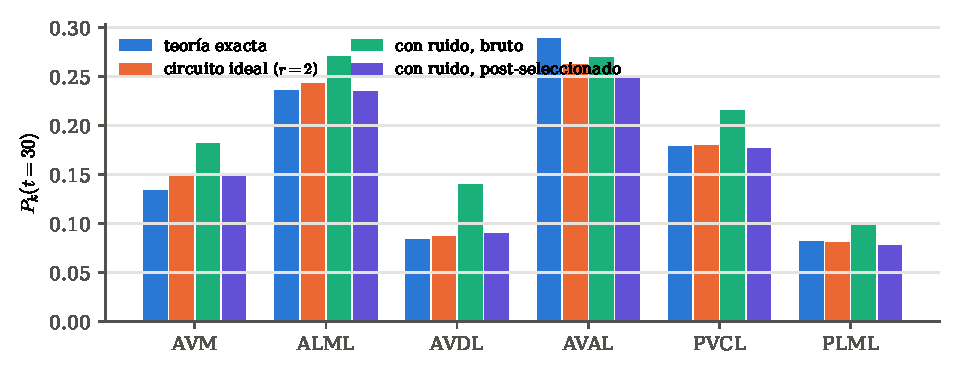
\includegraphics[width=\textwidth]{figuras/fig_postseleccion.pdf}
\caption{\code{toque-6}, $t=30$, $r=2$. Marginales de la teoría exacta, del circuito ideal (solo error de Trotter), del circuito con ruido tipo Forte en bruto y post-seleccionado. La post-selección baja la TVD respecto de la teoría de $0.21$ a $0.11$ conservando el $85\%$ de los shots.}
\label{fig:postseleccion}
\end{figure}

\paragraph{El costo.} Los shots útiles son $S\cdot f_{\text{acept}}$, así que el error estadístico crece en un factor $1/\sqrt{f_{\text{acept}}}$: con $f_{\text{acept}}=0.85$, apenas un $8\%$.

\subsection{Protocolo experimental}

\begin{enumerate}
\item Para cada tiempo del barrido se comparan cuatro curvas: (i) teoría exacta, (ii) circuito ideal, (iii) simulador de IonQ con modelo de ruido de Forte y (iv) hardware. Por \eqref{eq:triangular}, la diferencia (i)--(ii) es algorítmica y la (ii)--(iv) es de hardware.
\item Se usa el mismo $r$ para todos los tiempos.
\item Primero se corre en el simulador remoto de IonQ, que es gratis, y solo después en el hardware, que consume créditos.
\item Se informa la TVD bruta y la post-seleccionada junto con la fracción aceptada.
\end{enumerate}

% =====================================================================
\section{Verificación numérica}
\label{sec:verificacion}
% =====================================================================

Cada afirmación de este documento tiene una prueba automática que la comprueba.

\begin{center}
\renewcommand{\arraystretch}{1.15}
\begin{tabular}{@{}L{0.55\textwidth}L{0.38\textwidth}@{}}
\toprule
\textbf{Afirmación} & \textbf{Dónde se comprueba}\\
\midrule
$J$ simétrica, $\lVert J\rVert_2=1$, 302 neuronas (\cref{prop:norma}) & \code{test\_normalizacion}\\
Probabilidad total conservada en el walk & \code{test\_walk\_conserva\_norma}\\
Sector de 1 excitación de XY $=$ walk $\gamma J$ (\cref{prop:ctqw,prop:central}) & \code{test\_xy\_igual\_a\_walk}\\
Error de Trotter decrece con $r$ (\cref{prop:trotter}) & \code{test\_trotter\_converge}\\
Givens reproduce la distribución exacta (\cref{prop:givens}) & \code{test\_givens\_exacto}\\
Post-selección correcta & \code{test\_postseleccion}\\
Orden de bits de Qiskit ($q_0$ a la derecha) & \code{test\_orden\_de\_bits\_qiskit}\\
Un solo job con varios tiempos & \code{test\_ejecutar\_un\_solo\_job\_}\newline\code{varios\_tiempos}\\
Identidades de compilación nativa de IonQ & \code{backend/tests/}\newline\code{test\_compilation.py}\\
Ruido estratificado $=$ matriz densidad exacta & \code{backend/tests/}\newline\code{test\_trotter.py}\\
\bottomrule
\end{tabular}
\end{center}

% =====================================================================
\section{Límites y extensiones}
\label{sec:extensiones}
% =====================================================================

\begin{itemize}
\item \textbf{Sinapsis dirigidas.} Un hamiltoniano no puede ser asimétrico. Hay dos salidas. La primera son las fases complejas $J_{ij}\e^{\ii\varphi_{ij}}$, que rompen la simetría de inversión temporal y producen transporte direccional (\emph{chiral quantum walks}~\cite{zimboras2013}). La segunda es una caminata cuántica estocástica, que interpola entre el walk cuántico y el clásico con una ecuación de Lindblad~\cite{whitfield2010}:
\begin{equation}
\dot\rho=-(1-\omega)\,\ii[H,\rho]+\omega\sum_{ij}\Bigl(L_{ij}\rho L_{ij}^\dagger-\tfrac12\{L_{ij}^\dagger L_{ij},\rho\}\Bigr),\quad L_{ij}=\sqrt{W_{i\leftarrow j}}\,\ket{e_i}\!\bra{e_j}.
\end{equation}
\item \textbf{Inhibición.} Las sinapsis inhibitorias (por ejemplo GABAérgicas) podrían llevar signo negativo en $J_{ij}$. El circuito no cambia, porque los ángulos negativos ya se compilan.
\item \textbf{Disipación.} Un canal de \emph{amplitude damping} controlado modelaría el retorno de la neurona al reposo.
\item \textbf{Varios láseres en hardware.} Es el régimen de muchos cuerpos ($\binom nk$ estados, \cref{subsec:varios-laseres}) donde la simulación cuántica tiene sentido real. El modo Trotter ya lo soporta.
\item \textbf{Ver la coherencia.} Medir algunos qubits en base $X$ revelaría la superposición entre vacío y excitación, que la base $Z$ no ve.
\end{itemize}

% =====================================================================
\appendix
\section{Identidades de Pauli usadas}
\label{app:pauli}
% =====================================================================

\begin{equation}
X=\begin{pmatrix}0&1\\1&0\end{pmatrix},\quad
Y=\begin{pmatrix}0&-\ii\\\ii&0\end{pmatrix},\quad
Z=\begin{pmatrix}1&0\\0&-1\end{pmatrix},
\end{equation}
\begin{equation}
X^2=Y^2=Z^2=\mathbb 1,\qquad XY=\ii Z,\quad YZ=\ii X,\quad ZX=\ii Y,\qquad
\{P,Q\}=0\ \text{si}\ P\ne Q.
\end{equation}

Para cualquier Pauli $P$ (con $P^2=\mathbb 1$), $\e^{-\ii\alpha P/2}=\cos\frac\alpha2\,\mathbb 1-\ii\sin\frac\alpha2\,P$, y lo mismo para productos $P\otimes Q$. Rotar un Pauli $Q$ con otro $P$ que anticonmuta con él da
\begin{equation}
\e^{-\ii\theta P/2}\,Q\,\e^{\ii\theta P/2}=\cos\theta\,Q-\tfrac{\ii}{2}\sin\theta\,[P,Q].
\end{equation}

\section{Mapa entre ecuaciones y código}
\label{app:codigo}

\begin{center}
\renewcommand{\arraystretch}{1.15}
\begin{tabular}{@{}L{0.42\textwidth}L{0.52\textwidth}@{}}
\toprule
\textbf{Concepto} & \textbf{Función (\code{qollab/cerebro\_q})}\\
\midrule
Pesos y normalización \eqref{eq:pesos}, \eqref{eq:normalizacion} & \code{fisica.acoplamientos}\\
Descomposición espectral \eqref{eq:espectral} & \code{fisica.diagonalizacion}\\
Resultado central \eqref{eq:central} & \code{fisica.probabilidades\_walk}\\
Distribución exacta del microcircuito & \code{fisica.distribucion\_exacta}\\
Saltos de Trotter con fusión & \code{circuitos.saltos\_trotter}\\
Cascada de Givens (\cref{prop:givens}) & \code{circuitos.saltos\_givens}\\
Circuito de Qiskit & \code{circuitos.a\_qiskit}\\
Ruido estratificado y lectura & \code{circuitos.probabilidades\_con\_ruido}\\
$F_{hw}$ y conteo de compuertas & \code{circuitos.recursos}\\
Post-selección, marginales, TVD & \code{analisis.*}\\
Elección de $r^*$ & \code{api.\_autoajuste}\\
Ejecución en el backend (un job) & \code{api.ejecutar\_json}\\
\bottomrule
\end{tabular}
\end{center}

\section{Parámetros de la interfaz}

\begin{center}
\renewcommand{\arraystretch}{1.15}
\begin{tabular}{@{}lL{0.72\textwidth}@{}}
\toprule
$\theta$ & Ángulo del pulso; $P(\text{disparo})=\sin^2(\theta/2)$. Solo escala la respuesta.\\
$\gamma$ & Escala del acoplamiento. Cambiar $\gamma$ equivale a reescalar el tiempo ($\gamma t$ es lo único que importa).\\
$t$ & Tiempo de evolución, en unidades de $1/\gamma$.\\
$r$ & Pasos de Trotter (automático: $r^*$).\\
Modo & Trotter (simulación genuina) o Givens (preparación exacta, profundidad mínima).\\
Shots & Repeticiones del circuito; error estadístico $\le1/(2\sqrt S)$.\\
\bottomrule
\end{tabular}
\end{center}

% =====================================================================
\begin{thebibliography}{99}
\bibitem{farhi1998} E.~Farhi y S.~Gutmann, \emph{Quantum computation and decision trees}, Phys.\ Rev.\ A \textbf{58}, 915 (1998).
\bibitem{childs2009} A.~M.~Childs, \emph{Universal computation by quantum walk}, Phys.\ Rev.\ Lett.\ \textbf{102}, 180501 (2009).
\bibitem{mulken2011} O.~Mülken y A.~Blumen, \emph{Continuous-time quantum walks: models for coherent transport on complex networks}, Phys.\ Rep.\ \textbf{502}, 37 (2011).
\bibitem{cook2019} S.~J.~Cook \emph{et al.}, \emph{Whole-animal connectomes of both Caenorhabditis elegans sexes}, Nature \textbf{571}, 63 (2019).
\bibitem{white1986} J.~G.~White, E.~Southgate, J.~N.~Thomson y S.~Brenner, \emph{The structure of the nervous system of the nematode C.~elegans}, Phil.\ Trans.\ R.\ Soc.\ B \textbf{314}, 1 (1986).
\bibitem{chalfie1985} M.~Chalfie \emph{et al.}, \emph{The neural circuit for touch sensitivity in Caenorhabditis elegans}, J.\ Neurosci.\ \textbf{5}, 956 (1985).
\bibitem{nagel2005} G.~Nagel \emph{et al.}, \emph{Light activation of channelrhodopsin-2 in excitable cells of Caenorhabditis elegans triggers rapid behavioral responses}, Curr.\ Biol.\ \textbf{15}, 2279 (2005).
\bibitem{boyden2005} E.~S.~Boyden \emph{et al.}, \emph{Millisecond-timescale, genetically targeted optical control of neural activity}, Nat.\ Neurosci.\ \textbf{8}, 1263 (2005).
\bibitem{lloyd1996} S.~Lloyd, \emph{Universal quantum simulators}, Science \textbf{273}, 1073 (1996).
\bibitem{childs2021} A.~M.~Childs, Y.~Su, M.~C.~Tran, N.~Wiebe y S.~Zhu, \emph{Theory of Trotter error with commutator scaling}, Phys.\ Rev.\ X \textbf{11}, 011020 (2021).
\bibitem{kivlichan2018} I.~D.~Kivlichan \emph{et al.}, \emph{Quantum simulation of electronic structure with linear depth and connectivity}, Phys.\ Rev.\ Lett.\ \textbf{120}, 110501 (2018).
\bibitem{bonet2018} X.~Bonet-Monroig, R.~Sagastizabal, M.~Singh y T.~E.~O'Brien, \emph{Low-cost error mitigation by symmetry verification}, Phys.\ Rev.\ A \textbf{98}, 062339 (2018).
\bibitem{mcardle2019} S.~McArdle, X.~Yuan y S.~Benjamin, \emph{Error-mitigated digital quantum simulation}, Phys.\ Rev.\ Lett.\ \textbf{122}, 180501 (2019).
\bibitem{whitfield2010} J.~D.~Whitfield, C.~A.~Rodríguez-Rosario y A.~Aspuru-Guzik, \emph{Quantum stochastic walks}, Phys.\ Rev.\ A \textbf{81}, 022323 (2010).
\bibitem{zimboras2013} Z.~Zimborás \emph{et al.}, \emph{Quantum transport enhancement by time-reversal symmetry breaking}, Sci.\ Rep.\ \textbf{3}, 2361 (2013).
\bibitem{ionqnative} IonQ, \emph{Getting started with native gates}, \url{https://docs.ionq.com/guides/getting-started-with-native-gates}.
\bibitem{ionqbest} IonQ, \emph{Best practices for using IonQ hardware}, \url{https://ionq.com/docs/best-practices-for-using-ionq-hardware}.
\bibitem{ionqcompare} IonQ, \emph{Compare quantum systems}, \url{https://www.ionq.com/quantum-systems/compare}.
\bibitem{openworm} OpenWorm, \url{https://github.com/openworm/c302} y \url{https://github.com/openworm/CElegansNeuroML}.
\end{thebibliography}

\end{document}
